\documentclass{beamer}
\usefonttheme[onlymath]{serif}
\usepackage[T1]{fontenc}
\usepackage[utf8]{inputenc}
\usepackage[english]{babel}
\usepackage{amsmath}
\usepackage{amssymb}
\usepackage{amsthm}
\usepackage{gensymb}
\usepackage{parskip}
\usepackage{mathtools}
\usepackage{listings}
\usepackage{hyperref}
\usepackage{graphicx}
\usepackage{color}
\usepackage{enumerate}
\usepackage{verbatim}
\usepackage{minted}
\parskip 0pt


\DeclareMathOperator{\lcm}{lcm}
\newcommand\floor[1]{\left\lfloor#1\right\rfloor}
\newcommand\ceil[1]{\left\lceil#1\right\rceil}
\newcommand\abs[1]{\left|#1\right|}
\newcommand\p[1]{\left(#1\right)}
\newcommand\sqp[1]{\left[#1\right]}
\newcommand\cp[1]{\left\{#1\right\}}
\newcommand\norm[1]{\left\lVert#1\right\rVert}
\renewcommand\Im{\operatorname{Im}}
\renewcommand\Re{\operatorname{Re}}

\usetheme{metropolis}
\graphicspath{{../../shared/}}

\definecolor{dark yellow}{rgb} {0.6,0.6,0.0}
\definecolor{dark green}{rgb} {0.0,0.6,0.0}

\title{Number Theory}
\author{Atli FF}
\institute{\href{http://ru.is/td}{School of Computer Science} \\[2pt] \href{http://ru.is}{Reykjavík University}}
\titlegraphic{\hfill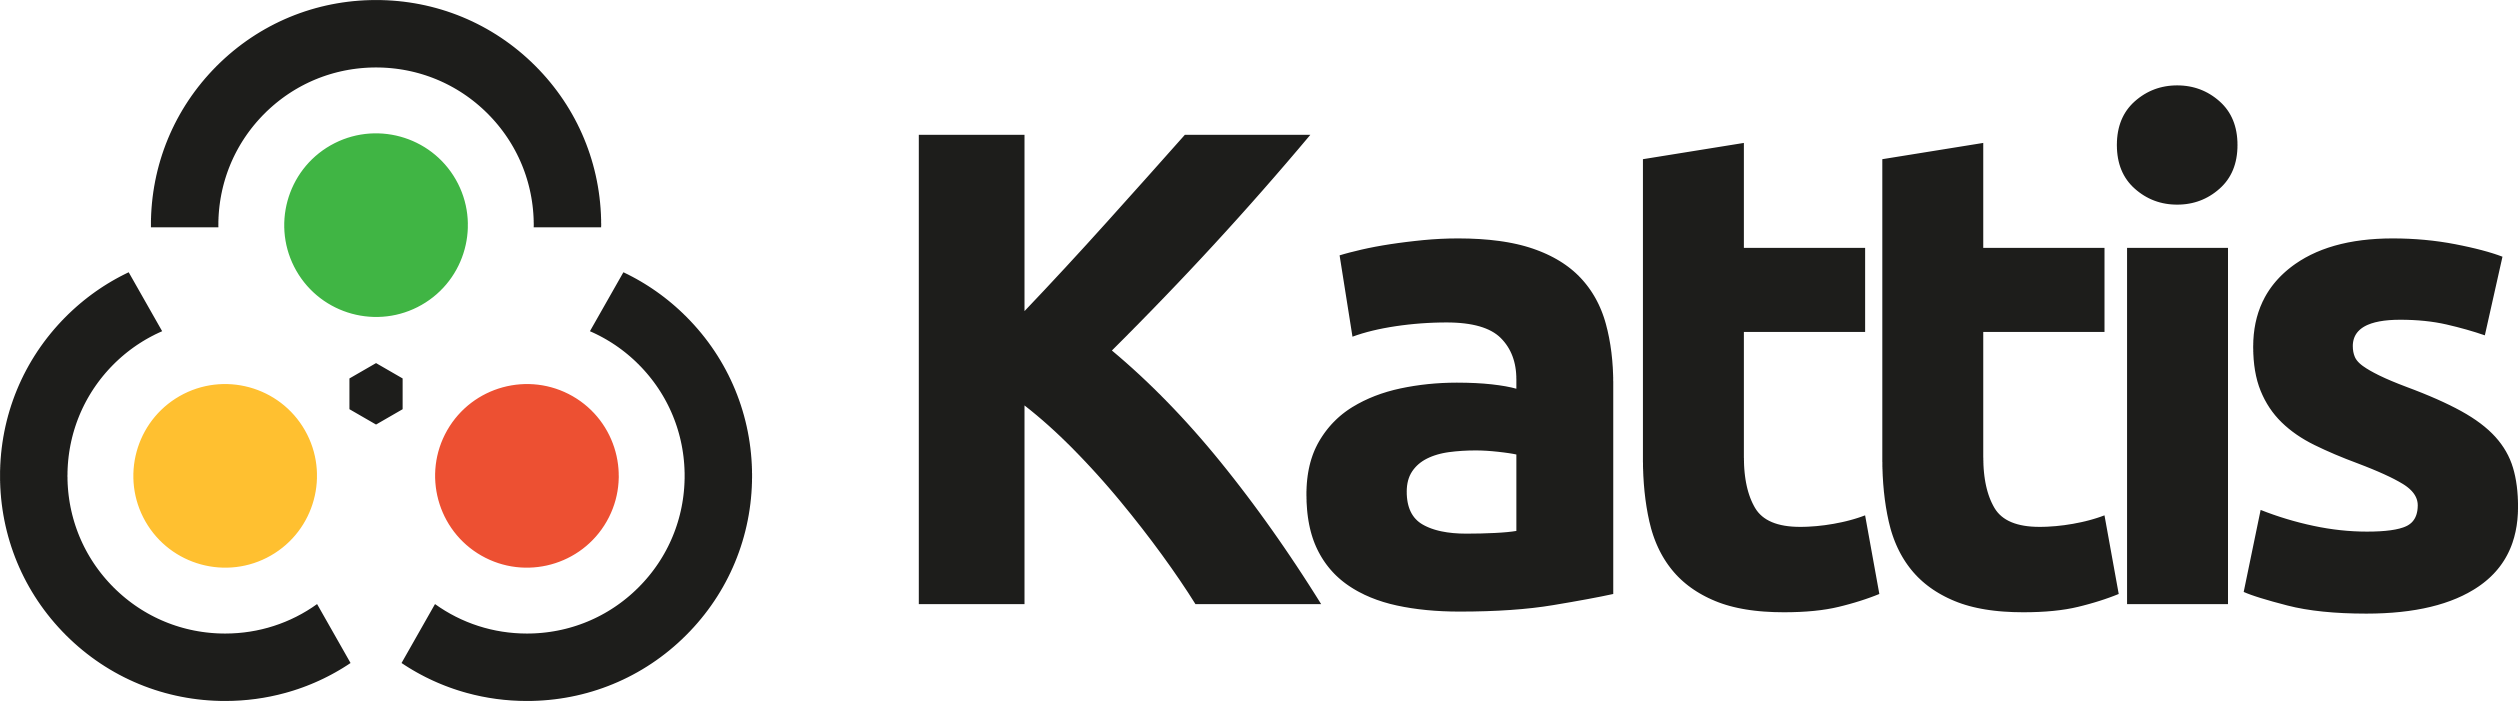
\includegraphics[height=0.6cm]{../shared/kattis}}
\date{\textbf{Árangursrík forritun og lausn verkefna}}

\begin{document}

\begin{frame}[plain]
    \titlepage
\end{frame}

\section*{Mathematical introduction}

\begin{frame}[plain]{Important point}
    \begin{center}
        Computer Science $\subset$ Mathematics
    \end{center}
    \vspace{10pt}
    \begin{itemize}
        \item Problems often require mathematical analysis to be solved efficiently.
        \item Using a bit of math before coding can also shorten and simplify code.
    \end{itemize}
\end{frame}

\begin{frame}[plain]{Pattern finding}
    \vspace{20pt}
    \begin{itemize}
        \item Some problems have solutions that form a pattern.
        \onslide<2-> \item By finding the pattern, we solve the problem.
        \item Could be classified as mathematical ad-hoc problem.
        \item Requires mathematical intuition.
        \onslide<3->{
            \item Useful tricks:
            \begin{itemize}
                \item Solve some small instances by hand.
                \item See if the solutions form a pattern.
            \end{itemize}
        } \onslide<4-> {
            \item Does the pattern involve some overlapping subproblem? \\
        } \onslide<5-> {
            We might need to use {\color{blue}DP}.
        } \onslide<6-> {
            \item Knowing reoccurring identities and sequences can be helpful.
        }
    \end{itemize}
\end{frame}

\begin{frame}[plain]{Arithmetic progression}
  \vspace{30pt}
  \begin{itemize}
    \item Often we see a pattern like
      \[
        2 , 5 , 8 , 11 , 14, 17, 20, \ldots
      \]
    \onslide<2->
    \item This is called an arithmetic progression.
      \[
        a_n = a_{n-1} + c
      \]
  \end{itemize}
\end{frame}

\begin{frame}[plain]{Arithmetic progression}
  \vspace{30pt}
  \begin{itemize}
    \item Depending on the situation we may want to get the $n$-th element
      \[
        a_n = a_1 + (n-1) c
      \]
    \item Or the sum over a finite portion of the progression
      \[
        S_n = \frac{n(a_1 + a_n)}{2}
      \]
    \onslide<2->
    \item Remember this one?
      \[
        1 + 2 + 3 + 4 + 5 + \ldots + n = \frac{n(n+1)}{2}
      \]
  \end{itemize}
\end{frame}

\begin{frame}[plain]{Geometric progression}
  \vspace{30pt}
  \begin{itemize}
    \item Other types of pattern we often see are geometric progressions
      \[
        1,\, 2,\, 4,\, 8,\, 16,\, 32,\, 64,\, 128,\, \ldots
      \]
    \onslide<2->{
      \item More generally
        \[
          s,\, sr,\, sr^2,\, sr^3,\, sr^4,\, sr^5,\, sr^6,\, \ldots
        \]
        \[
          a_n  = s r^{n-1}
        \]
      }
  \end{itemize}
\end{frame}

\begin{frame}[plain]{Geometric progression}
  \vspace{30pt}
  \begin{itemize}
    \item Sum over a finite portion
      \[
        \sum_{i = 0}^n sr^i =  \frac{s(1-r^n)}{(1-r)}
      \]
    \onslide<2->{
      \item Or from the $m$-th element to the $n$-th
        \[
          \sum_{i = m}^n sr^i =  \frac{s(r^{m}-r^{n+1})}{(1-r)}
        \]
    }
  \end{itemize}
\end{frame}

\begin{frame}[plain,fragile]{Quick note on logarithms}
  \vspace{30pt}
  \begin{itemize}
    \item Sometimes doing computation in logarithm can be an efficient alternative.

    \onslide<2->
  \item In both C++(\texttt{<cmath>}) and
    Java(\texttt{java.lang.Math}) we have the natural logarithm
      \begin{minted}{cpp}
    double log(double x);
      \end{minted}

    \onslide<3->
      and logarithm in base $10$
      \begin{minted}{cpp}
    double log10(double x);
      \end{minted}
    \onslide<4->
  \item And also the exponential
    \begin{minted}{cpp}
    double exp(double x);
    \end{minted}
  \end{itemize}
\end{frame}

\begin{frame}[plain,fragile]{Example}
  \vspace{20pt}
  \begin{itemize}
    \item For example, what is the first power of $17$ that has $k$ digits in base $b$?
    \onslide<2->
    \item Naive solution: Iterate over powers of $17$ and count the number of digits.
    \onslide<3->
    \item But the powers of $17$ grow exponentially!
      \[17^{16} > 2^{64}\]
    \item What if $k = 500$ ($\sim1.7 \cdot 10^{615}$), or something larger?
    \onslide<4->
    \item Impossible to work with the numbers in a normal fashion.
    \item Why not $\log$?
  \end{itemize}
\end{frame}

\begin{frame}[plain,fragile]{Example}
  \vspace{40pt}
  \begin{itemize}
    \item Remember, we can calculate the length of a number $n$ in base $b$
      with $\lfloor \log_b(n) \rfloor + 1$.
    \onslide<2->
    \item But how do we do this with only $\ln$ or $\log_{10}$?
    \onslide<3->
    \item Change base!
      \[
        \log_b(a) = \frac{\log_d(a)}{\log_d(b)} = \frac{\ln(a)}{\ln(b)}
      \]
    \item Now we can at least count the length without converting bases
  \end{itemize}
\end{frame}

\begin{frame}[plain]{Example}
  \vspace{20pt}
  \begin{itemize}
    \item We still have to iterate over the powers of $17$, but we can do that in log
      \[
        \ln(17^{x-1} \cdot 17) = \ln(17^{x-1}) + \ln(17)
      \]
    \onslide<2->
    \item More generally
      \[
        \log_b(xy) = \log_b(x) + \log_b(y)
      \]
    \item For division
      \[
        \log_b\p{\frac{x}{y}} = \log_b(x) - \log_b(y)
      \]
  \end{itemize}
\end{frame}

\begin{frame}[plain]{Example}
  \vspace{20pt}
  \begin{itemize}
    \item We can simplify this even more.
    \item The solution to our problem is in mathematical terms, finding the $x$ for
      \[
        \log_b(17^x) = k - 1
      \]
    \onslide<2->
    \item One more handy identity
      \[
        \log_b(a^c) = c \cdot \log_b(a)
      \]
    \onslide<3->
    \item Using this identity and the ones we've covered, we get
      \[
        x = \left\lceil (k-1) \cdot \frac{\ln(10)}{\ln(17)} \right\rceil
      \]
  \end{itemize}
\end{frame}

\begin{frame}[plain,fragile]
  \frametitle{Base conversion}
  \begin{itemize}
    \item Speaking of bases.
    \onslide<2->
    \item What if we actually need to use base conversion?
    \onslide<3->
    \item Simple algorithm
      \begin{minted}{cpp}
vector<int> toBase(int base, int val) {
    vector<int> res;
    while(val) {
        res.push_back(val % base);
        val /= base;
    }
    return val;
}
      \end{minted}
    \item Starts from the $0$-th digit, and calculates the multiple of each power.
  \end{itemize}
\end{frame}

\begin{frame}[plain,fragile]
  \frametitle{Working with doubles}
  \vspace{30pt}
  \begin{itemize}
    \item Comparing doubles, sounds like a bad idea.
  \onslide<2->
    \item What else can we do if we are working with real numbers?
  \onslide<3->
    \item We compare them to a certain degree of precision like in binary search.
  \onslide<4->
    \item Two numbers are deemed equal if their difference is less than some small epsilon.
  \end{itemize}

    \begin{minted}{cpp}
    const double EPS = 1e-9;

    if(abs(a - b) < EPS) {
    ...
    }
    \end{minted}
\end{frame}

\begin{frame}[plain,fragile]
  \frametitle{Working with doubles}
  \vspace{30pt}
  \begin{itemize}
    \item Less than operator:
      \begin{minted}{cpp}
    if(a < b - EPS) {
    ...
    }
      \end{minted}
    \item Less than or equal:
      \begin{minted}{cpp}
    if(a  < b + EPS) {
    ...
    }
    \end{minted}
    \item The rest of the operators follow.
  \end{itemize}
\end{frame}

\section*{Primes and factorization}

\begin{frame}[plain]{Definitions that everybody should know}
  \vspace{15pt}
  \begin{itemize}
    \item {\color{red}Prime number} is a positive integer greater than $1$
      that has no positive divisor other than $1$ and itself.
    \item {\color{red}Greatest Common Divisor} of two integers $a$ and $b$ is the
      largest number that divides both $a$ and $b$.
    \item {\color{red}Least Common Multiple} of two integers $a$ and $b$ is
      the smallest integer that both $a$ and $b$ divide.
  \end{itemize}
\end{frame}

\begin{frame}[plain]{Definitions that everybody should know}
  \vspace{15pt}
  \begin{itemize}
    \item Every positive integer $n$ can be factored as a product of primes
  \end{itemize}
\end{frame}

\begin{frame}[plain]{Primality checking}
  \vspace{20pt}
  \begin{itemize}
    \item How do we determine if a number $n$ is a prime?
    \onslide<2->
    \item {\color{dark green}Naive method:} Iterate over all $1 < i < n$ and check if
      $i$ divides $n$.
      \begin{itemize}
        \item  $O(N)$
      \end{itemize}
    \onslide<3->
    \item {\color{dark green}Better:} If $n$ is not a prime, it has a divisor $\leq \sqrt{n}$.
      \begin{itemize}
        \item Iterate up to $\sqrt{n}$ instead.
        \item $O(\sqrt{N})$
      \end{itemize}
  \end{itemize}
\end{frame}

\begin{frame}[plain,fragile]{$\mathcal{O}(\sqrt{n})$ check}
\begin{minted}{cpp}
bool is_prime(ll x) {
    if(x <= 1) return 0;
    for(ll i = 2; i * i <= x; ++i)
        if(x % i == 0)
            return false;
    return true;
}
\end{minted}
\end{frame}

\section*{Modular arithmetic}

\begin{frame}[plain,fragile]
  \frametitle{Modulo}
  \vspace{30pt}
  \begin{itemize}
    \item Problem statements often end with the sentence \\
      \vspace{10pt}
      \begin{quote}
``... and output the answer modulo n.''
      \end{quote}
      \vspace{10pt}
  \onslide<2->
    \item This implies that we can do all the computation with integers \emph{modulo }$n$.
  \onslide<3->
    \item But what does this mean? Taking an integer modulo $n$ means taking the remainder of it when we divide by $n$.
  \onslide<4->
    \item Thus if we do everything modulo $n$ we consider every number a multiple of $n$ apart the same. So modulo $7$ the numbers $1, 8, -6, 15, -13, \dots$ are all the same, and so are $5, -2, 12, -9, 19, \dots$.
  \end{itemize}
\end{frame}

\begin{frame}[plain,fragile]
  \frametitle{Modulo}
  \begin{itemize}
  \item In this system it's simplest if we pick one of the infinite set of equivalent numbers to be the one we use to represent them. We usually choose the representatives $0, 1, \dots, n - 1$ if we're working modulo $n$.
  \item<2-> Then to do addition, subtraction and multiplication we just do it as usual, but add or subtract multiples of $n$ afterwards so we end up back in $\{0, 1, \dots, n - 1\}$.
  \item<3-> This means this set, which we denote $\mathbb{Z}_n$, is a ring, for those familiar with that terminology.
  \end{itemize}
\end{frame}

\begin{frame}[plain,fragile]
  \frametitle{Modulo}
  \vspace{30pt}
  \begin{itemize}
    \item Problem statements often end with the sentence \\
      \vspace{10pt}
      \begin{quote}
``... and output the answer modulo n.''
      \end{quote}
      \vspace{10pt}
  \onslide<2->
    \item This implies that we can do all the computation in $\mathbb{Z}_n$.
  \onslide<3->
    \item This is often very useful, since the numbers never get too big and we don't generally have to worry about over/underflow.
  \end{itemize}
\end{frame}

\begin{frame}[plain]
  \frametitle{Division}
  \vspace{30pt}
  \begin{itemize}
    \item What about division? Is it possible to divide? \onslide<2->{{\color{blue}Not always!}}
  \onslide<3->
    \item We could end up with a fraction!
    \item Division with $k$ equals multiplication with the \emph{multiplicative
      inverse} of $k$.
  \onslide<4->
    \item The \emph{multiplicative inverse} of an integer $a$, is the element $a^{-1}$ such that
      \[
        a \cdot a^{-1} = 1 \pmod{n}
      \]
   \item<5-> Such an $a^{-1}$ does not always exist, let's see how we can find it when it does exist though.
  \end{itemize}
\end{frame}

\begin{frame}[plain,fragile]{Euclidean algorithm}
  \vspace{20pt}
  \begin{itemize}
    \item The Euclidean algorithm is a recursive algorithm that computes the GCD of two numbers.
      \begin{minted}{cpp}
int gcd(int a, int b){
    return b == 0 ? a : gcd(b, a % b);
}
    \end{minted}
    \item Runs in $O(\log N)$.
    \onslide<2->
    \item Notice that this can also compute LCM
      \[
        \text{lcm}(a, b) = \frac{a\cdot b}{\gcd(a,b)}
      \]
    \item See Wikipedia to see how it works and for proofs.
  \end{itemize}
\end{frame}

\begin{frame}[plain]{Extended Euclidean algorithm}
  \vspace{20pt}
  \begin{itemize}
    \item Reversing the steps of the Euclidean algorithm we get the B\'ezout's identity
      \[
        \gcd(a, b) = ax + by
      \]
    which simply states that there always exist $x$ and $y$ such that the equation above holds.
    \onslide<2->
    \item The extended Euclidean algorithm computes the GCD and the coefficients $x$ and $y$.
    \item Each iteration it add up how much of $b$ we subtracted from $a$ and vice versa.
  \end{itemize}
\end{frame}

\begin{frame}[plain,fragile]{Extended Euclidean algorithm}
  \vspace{10pt}
    \begin{minted}{cpp}
int egcd(int a, int b, int& x, int& y) {
    if (b == 0) {
        x = 1;
        y = 0;
        return a;
    } else {
        int d = egcd(b, a % b, x, y);
        x -= a / b * y;
        swap(x, y);
        return d;
    }
}
    \end{minted}
\end{frame}

\begin{frame}[plain]{Applications}
  \vspace{40pt}
  \begin{itemize}
    \item Essential step in the RSA algorithm.
    \item Essential step in many factorization algorithms.
    \item Can be generalized to other algebraic structures.
    \item Fundamental tool for proofs in number theory.
    \item Many other algorithms for GCD
  \end{itemize}
\end{frame}

\begin{frame}[plain]{Modular inverse}
  \vspace{20pt}
  Back to modular inverse.
  \begin{itemize}
    \item Working modulo $n$ often requires division (multiplication by inverse).
    \onslide<2->
    \item Given some $a \pmod{n}$, then the multiplicative inverse $a^{-1}
      \pmod{n}$ exists iff. $a$ and $n$ are coprime.
    \onslide<3->
    \item It so happens that when we have from EGCD algorithm
      \[
        ax + ny = \gcd(a,n) = 1
      \]
      then \[ a^{-1} \equiv x \pmod{n} \]
  \end{itemize}
\end{frame}

\begin{frame}[plain, fragile]{Modular inverse}
    \begin{minted}{cpp}
int mod_inv(int a, int m) {
    int x, y, d = egcd(a, m, x, y);
    return d == 1 ? (x%m+m)%m : -1;
}
\end{minted}
\end{frame}

\begin{frame}[plain]
  \frametitle{Discrete logarithm}
  \vspace{30pt}
  \begin{itemize}
    \item What about logarithm? \onslide<2->{{\color{red}YES!}}
      \onslide<2->
      \begin{itemize}
        \item But difficult.
        \onslide<3->
        \item Basis for some cryptography such as elliptic curve, Diffie-Hellmann.
      \end{itemize}
    \item Google ``Discrete Logarithm'' if you want to know more.
  \end{itemize}
\end{frame}



\begin{frame}[plain]{Chinese remainder theorem}
  \vspace{20pt}
  What is the lowest number $n$ such that when divided by
  \vspace{10pt}
  \begin{itemize}
    \item[] ... $3$ it leaves $2$ in remainder.
    \item[] ... $5$ it leaves $3$ in remainder.
    \item[] ... $7$ it leaves $2$ in remainder.
  \end{itemize}
  \vspace{10pt}
  \onslide<2->
  When stated mathematically, find $n$ where
      \begin{align*}
  n &\equiv 2 \pmod{3} \\
  n &\equiv 3 \pmod{5} \\
  n &\equiv 2 \pmod{7}
      \end{align*}
\end{frame}

\begin{frame}[plain]{Chinese remainder theorem}
  \vspace{20pt}
  The Chinese remainder theorem states that:
  \begin{itemize}
    \item When the moduli of a system of linear congruences are pairwise
      coprime, there exists a unique solution modulo the product of the moduli.
  \end{itemize}
  \onslide<2->
  Let $n_1, n_2,\ldots, n_k$ be pairwise coprime positive integers, and let $x$
  be the solution to the system of linear congruences
  \begin{align*}
    x &\equiv  b_1 \pmod{n_1} \\
    x &\equiv  b_2 \pmod{n_2} \\
      &\vdots                 \\
    x &\equiv b_k \pmod{n_k}
  \end{align*}
\end{frame}

\begin{frame}[plain]{Chinese remainder theorem}
  \vspace{10pt}
  \begin{itemize}
    \item The Chinese remainder theorem only states that there exists a solution and it
  is unique modulus the product of the moduli. \\
    \item To obtain the solution $x$
      \[
        x \equiv b_1 c_1 \frac{N}{n_1} + \ldots + b_k c_k \frac{N}{n_k}
      \]
      where $N = n_1 n_2 \cdots n_k$.
    \item The coefficients $c_i$ are determined from
      \[
        c_i \frac{N}{n_i} \equiv 1 \pmod{n_i}
      \]
      (the multiplicative inverse of $\frac{N}{n_i}$ modulus $n_i$)
    \item Use EGCD to compute $c_i$.
  \end{itemize}
\end{frame}



\begin{frame}[plain]
\frametitle{Faster?}

\begin{itemize}
    \item Can we do this faster?
    \item Sort of.
    \item We can use probabilistic prime testing, a function that says the input is \textit{probably} prime.
    \item This may sound shaky, but this program can be run a dozen times and at that point the probability of the program being wrong every
        time is so vanishingly small you would spend your time better worrying about space rays flipping your bits while you run the program.
\end{itemize}

\end{frame}

\begin{frame}[plain]
\frametitle{Miller-Rabin concept}

\begin{itemize}

\item Let us first note that if $x^2 = 1 \ (mod \ p)$ this can be factored as $(x-1)(x+1) = 0 \ (mod \ p)$ and since $p$ is prime this means $x = \pm 1 \ (mod \ p)$.

\item Now take some $p > 2$ and $a < p$. Write $p - 1 = 2^sd$ s.t. $d$ is odd. Then by taking the square root on each side of the equation $a^{p - 1} = 1 \ (mod \ p)$ (which we know is true) then either the right side will at some point equal $-1$ and we have to stop, or we eventually divide out all powers of two in $a$. This either $a^d = 1 \ (mod \ p)$ or $a^{2^r d} = -1 \ (mod \ p)$ for some $0 \leq r \leq s - 1$.

\item Thus to prove that $n$ is not prime we try to find $a < n$ s.t. $a^d \neq 1 \ (mod \ n)$ and $a^{2^rd} \neq -1 \ (mod \ n)$ for all $0 \leq r \leq s - 1$.

\end{itemize}

\end{frame}

\begin{frame}[plain]
\frametitle{Miller-Rabin concept ctd.}

\begin{itemize}

    \item Finding such an $a$ sounds far fetched, but it turns out that a large percentage of numbers will work as the choice of $a$ if $n$ is not prime.
    \item Thus the Miller-Rabin algorithm works by choosing random $a$ and seeing if it excludes the possibility of $n$ being prime.

    \item Thus the algorithm is such that if it says $p$ is not prime, this is definitely true. If it says $p$ is a prime, it really means ``I couldn't exclude the possibility that $p$ is prime, but it could be non-prime''. 

    \item If we test many $a$ the odds are in our favor. Thus we let the program take a variable \texttt{it} saying how often it should run. This runs in $\mathcal{O}(it\log(n)^3)$ for large $n$.

\end{itemize}

\end{frame}

\begin{frame}[plain, fragile]
\frametitle{Miller-Rabin implementation}

\begin{small}
\begin{minted}{cpp}
bool isprobablyprime(ll n, int it) {
    if(n % 2 == 0) return n == 2;
    if(n <= 3) return n == 3;
    ll d = n - 1, r = 0;
    while(d % 2 == 0) d >>= 1, r++;
    for(int i = 0; i < it; ++i) {
        ll a = (n - 3) * rand() / RAND_MAX + 2;
        ll x = modpow(a, d, n);
        if(x == 1 || x == n - 1) continue;
        for(ll j = 0; j < r - 1; ++j) {
            x = (x * x % n + n) % n;
            if(x == n - 1) continue;
        }
        return false;
    }
    return true;
}
\end{minted}
\end{small}

\end{frame}

\begin{frame}[plain,fragile]{Bulk discount}
  \begin{itemize}
    \item If we want to generate primes, using a primality test is very inefficient.
    \onslide<2->
    \item Instead, our preferred method of prime generation is the sieve of Eratosthenes.
      \begin{itemize}
        \onslide<3->
        \item For all numbers from $2$ to $\sqrt{n}$:
        \onslide<4->
        \item If the number is not marked, iterate over every multiple of the
          number up to $n$ and mark them.
        \onslide<5->
        \item The unmarked numbers are those that are not a multiple of any
          smaller number.
        \item $O(N\log \log N)$
      \end{itemize}
  \end{itemize}
\end{frame}

\begin{frame}[plain]{Eratosthenes example}
	\only<all:1> {
		\begin{tabular}{r r r r r r r r r r}
			\color{black}  $0$ & \color{black}  $1$ & \color{black}  $2$ & \color{black}  $3$ & \color{black}  $4$ & \color{black}  $5$ & \color{black}  $6$ & \color{black}  $7$ & \color{black}  $8$ & \color{black}  $9$\\
			\color{black} $10$ & \color{black} $11$ & \color{black} $12$ & \color{black} $13$ & \color{black} $14$ & \color{black} $15$ & \color{black} $16$ & \color{black} $17$ & \color{black} $18$ & \color{black} $19$\\
			\color{black} $20$ & \color{black} $21$ & \color{black} $22$ & \color{black} $23$ & \color{black} $24$ & \color{black} $25$ & \color{black} $26$ & \color{black} $27$ & \color{black} $28$ & \color{black} $29$\\
			\color{black} $30$ & \color{black} $31$ & \color{black} $32$ & \color{black} $33$ & \color{black} $34$ & \color{black} $35$ & \color{black} $36$ & \color{black} $37$ & \color{black} $38$ & \color{black} $39$\\
			\color{black} $40$ & \color{black} $41$ & \color{black} $42$ & \color{black} $43$ & \color{black} $44$ & \color{black} $45$ & \color{black} $46$ & \color{black} $47$ & \color{black} $48$ & \color{black} $49$\\
			\color{black} $50$ & \color{black} $51$ & \color{black} $52$ & \color{black} $53$ & \color{black} $54$ & \color{black} $55$ & \color{black} $56$ & \color{black} $57$ & \color{black} $58$ & \color{black} $59$\\
			\color{black} $60$ & \color{black} $61$ & \color{black} $62$ & \color{black} $63$ & \color{black} $64$ & \color{black} $65$ & \color{black} $66$ & \color{black} $67$ & \color{black} $68$ & \color{black} $69$\\
			\color{black} $70$ & \color{black} $71$ & \color{black} $72$ & \color{black} $73$ & \color{black} $74$ & \color{black} $75$ & \color{black} $76$ & \color{black} $77$ & \color{black} $78$ & \color{black} $79$\\
			\color{black} $80$ & \color{black} $81$ & \color{black} $82$ & \color{black} $83$ & \color{black} $84$ & \color{black} $85$ & \color{black} $86$ & \color{black} $87$ & \color{black} $88$ & \color{black} $89$\\
			\color{black} $90$ & \color{black} $91$ & \color{black} $92$ & \color{black} $93$ & \color{black} $94$ & \color{black} $95$ & \color{black} $96$ & \color{black} $97$ & \color{black} $98$ & \color{black} $99$\\
			\phantom{$888$} & \phantom{$888$} & \phantom{$888$} & \phantom{$888$} & \phantom{$888$} & \phantom{$888$} & \phantom{$888$} & \phantom{$888$} & \phantom{$888$} & \phantom{$888$}
        \end{tabular}
    }
	\only<all:2> {
		\begin{tabular}{r r r r r r r r r r}
			                   &                    & \color{black}  $2$ & \color{black}  $3$ & \color{black}  $4$ & \color{black}  $5$ & \color{black}  $6$ & \color{black}  $7$ & \color{black}  $8$ & \color{black}  $9$\\
			\color{black} $10$ & \color{black} $11$ & \color{black} $12$ & \color{black} $13$ & \color{black} $14$ & \color{black} $15$ & \color{black} $16$ & \color{black} $17$ & \color{black} $18$ & \color{black} $19$\\
			\color{black} $20$ & \color{black} $21$ & \color{black} $22$ & \color{black} $23$ & \color{black} $24$ & \color{black} $25$ & \color{black} $26$ & \color{black} $27$ & \color{black} $28$ & \color{black} $29$\\
			\color{black} $30$ & \color{black} $31$ & \color{black} $32$ & \color{black} $33$ & \color{black} $34$ & \color{black} $35$ & \color{black} $36$ & \color{black} $37$ & \color{black} $38$ & \color{black} $39$\\
			\color{black} $40$ & \color{black} $41$ & \color{black} $42$ & \color{black} $43$ & \color{black} $44$ & \color{black} $45$ & \color{black} $46$ & \color{black} $47$ & \color{black} $48$ & \color{black} $49$\\
			\color{black} $50$ & \color{black} $51$ & \color{black} $52$ & \color{black} $53$ & \color{black} $54$ & \color{black} $55$ & \color{black} $56$ & \color{black} $57$ & \color{black} $58$ & \color{black} $59$\\
			\color{black} $60$ & \color{black} $61$ & \color{black} $62$ & \color{black} $63$ & \color{black} $64$ & \color{black} $65$ & \color{black} $66$ & \color{black} $67$ & \color{black} $68$ & \color{black} $69$\\
			\color{black} $70$ & \color{black} $71$ & \color{black} $72$ & \color{black} $73$ & \color{black} $74$ & \color{black} $75$ & \color{black} $76$ & \color{black} $77$ & \color{black} $78$ & \color{black} $79$\\
			\color{black} $80$ & \color{black} $81$ & \color{black} $82$ & \color{black} $83$ & \color{black} $84$ & \color{black} $85$ & \color{black} $86$ & \color{black} $87$ & \color{black} $88$ & \color{black} $89$\\
			\color{black} $90$ & \color{black} $91$ & \color{black} $92$ & \color{black} $93$ & \color{black} $94$ & \color{black} $95$ & \color{black} $96$ & \color{black} $97$ & \color{black} $98$ & \color{black} $99$\\
			\phantom{$888$} & \phantom{$888$} & \phantom{$888$} & \phantom{$888$} & \phantom{$888$} & \phantom{$888$} & \phantom{$888$} & \phantom{$888$} & \phantom{$888$} & \phantom{$888$}
        \end{tabular}
	}
	\only<all:3> {
		\begin{tabular}{r r r r r r r r r r}
			                   &                    & \color{ blue}  $2$ & \color{black}  $3$ & \color{black}  $4$ & \color{black}  $5$ & \color{black}  $6$ & \color{black}  $7$ & \color{black}  $8$ & \color{black}  $9$\\
			\color{black} $10$ & \color{black} $11$ & \color{black} $12$ & \color{black} $13$ & \color{black} $14$ & \color{black} $15$ & \color{black} $16$ & \color{black} $17$ & \color{black} $18$ & \color{black} $19$\\
			\color{black} $20$ & \color{black} $21$ & \color{black} $22$ & \color{black} $23$ & \color{black} $24$ & \color{black} $25$ & \color{black} $26$ & \color{black} $27$ & \color{black} $28$ & \color{black} $29$\\
			\color{black} $30$ & \color{black} $31$ & \color{black} $32$ & \color{black} $33$ & \color{black} $34$ & \color{black} $35$ & \color{black} $36$ & \color{black} $37$ & \color{black} $38$ & \color{black} $39$\\
			\color{black} $40$ & \color{black} $41$ & \color{black} $42$ & \color{black} $43$ & \color{black} $44$ & \color{black} $45$ & \color{black} $46$ & \color{black} $47$ & \color{black} $48$ & \color{black} $49$\\
			\color{black} $50$ & \color{black} $51$ & \color{black} $52$ & \color{black} $53$ & \color{black} $54$ & \color{black} $55$ & \color{black} $56$ & \color{black} $57$ & \color{black} $58$ & \color{black} $59$\\
			\color{black} $60$ & \color{black} $61$ & \color{black} $62$ & \color{black} $63$ & \color{black} $64$ & \color{black} $65$ & \color{black} $66$ & \color{black} $67$ & \color{black} $68$ & \color{black} $69$\\
			\color{black} $70$ & \color{black} $71$ & \color{black} $72$ & \color{black} $73$ & \color{black} $74$ & \color{black} $75$ & \color{black} $76$ & \color{black} $77$ & \color{black} $78$ & \color{black} $79$\\
			\color{black} $80$ & \color{black} $81$ & \color{black} $82$ & \color{black} $83$ & \color{black} $84$ & \color{black} $85$ & \color{black} $86$ & \color{black} $87$ & \color{black} $88$ & \color{black} $89$\\
			\color{black} $90$ & \color{black} $91$ & \color{black} $92$ & \color{black} $93$ & \color{black} $94$ & \color{black} $95$ & \color{black} $96$ & \color{black} $97$ & \color{black} $98$ & \color{black} $99$\\
			\phantom{$888$} & \phantom{$888$} & \phantom{$888$} & \phantom{$888$} & \phantom{$888$} & \phantom{$888$} & \phantom{$888$} & \phantom{$888$} & \phantom{$888$} & \phantom{$888$}
        \end{tabular}
	}
	\only<all:4> {
		\begin{tabular}{r r r r r r r r r r}
			                   &                    & \color{ blue}  $2$ & \color{black}  $3$ & \color{  red}  $4$ & \color{black}  $5$ & \color{  red}  $6$ & \color{black}  $7$ & \color{  red}  $8$ & \color{black}  $9$\\
			\color{  red} $10$ & \color{black} $11$ & \color{  red} $12$ & \color{black} $13$ & \color{  red} $14$ & \color{black} $15$ & \color{  red} $16$ & \color{black} $17$ & \color{  red} $18$ & \color{black} $19$\\
			\color{  red} $20$ & \color{black} $21$ & \color{  red} $22$ & \color{black} $23$ & \color{  red} $24$ & \color{black} $25$ & \color{  red} $26$ & \color{black} $27$ & \color{  red} $28$ & \color{black} $29$\\
			\color{  red} $30$ & \color{black} $31$ & \color{  red} $32$ & \color{black} $33$ & \color{  red} $34$ & \color{black} $35$ & \color{  red} $36$ & \color{black} $37$ & \color{  red} $38$ & \color{black} $39$\\
			\color{  red} $40$ & \color{black} $41$ & \color{  red} $42$ & \color{black} $43$ & \color{  red} $44$ & \color{black} $45$ & \color{  red} $46$ & \color{black} $47$ & \color{  red} $48$ & \color{black} $49$\\
			\color{  red} $50$ & \color{black} $51$ & \color{  red} $52$ & \color{black} $53$ & \color{  red} $54$ & \color{black} $55$ & \color{  red} $56$ & \color{black} $57$ & \color{  red} $58$ & \color{black} $59$\\
			\color{  red} $60$ & \color{black} $61$ & \color{  red} $62$ & \color{black} $63$ & \color{  red} $64$ & \color{black} $65$ & \color{  red} $66$ & \color{black} $67$ & \color{  red} $68$ & \color{black} $69$\\
			\color{  red} $70$ & \color{black} $71$ & \color{  red} $72$ & \color{black} $73$ & \color{  red} $74$ & \color{black} $75$ & \color{  red} $76$ & \color{black} $77$ & \color{  red} $78$ & \color{black} $79$\\
			\color{  red} $80$ & \color{black} $81$ & \color{  red} $82$ & \color{black} $83$ & \color{  red} $84$ & \color{black} $85$ & \color{  red} $86$ & \color{black} $87$ & \color{  red} $88$ & \color{black} $89$\\
			\color{  red} $90$ & \color{black} $91$ & \color{  red} $92$ & \color{black} $93$ & \color{  red} $94$ & \color{black} $95$ & \color{  red} $96$ & \color{black} $97$ & \color{  red} $98$ & \color{black} $99$\\
			\phantom{$888$} & \phantom{$888$} & \phantom{$888$} & \phantom{$888$} & \phantom{$888$} & \phantom{$888$} & \phantom{$888$} & \phantom{$888$} & \phantom{$888$} & \phantom{$888$}
        \end{tabular}
	}
	\only<all:5> {
		\begin{tabular}{r r r r r r r r r r}
			                   &                    & \color{ blue}  $2$ & \color{black}  $3$ &                    & \color{black}  $5$ &                    & \color{black}  $7$ &                    & \color{black}  $9$\\
			                   & \color{black} $11$ &                    & \color{black} $13$ &                    & \color{black} $15$ &                    & \color{black} $17$ &                    & \color{black} $19$\\
			                   & \color{black} $21$ &                    & \color{black} $23$ &                    & \color{black} $25$ &                    & \color{black} $27$ &                    & \color{black} $29$\\
			                   & \color{black} $31$ &                    & \color{black} $33$ &                    & \color{black} $35$ &                    & \color{black} $37$ &                    & \color{black} $39$\\
			                   & \color{black} $41$ &                    & \color{black} $43$ &                    & \color{black} $45$ &                    & \color{black} $47$ &                    & \color{black} $49$\\
			                   & \color{black} $51$ &                    & \color{black} $53$ &                    & \color{black} $55$ &                    & \color{black} $57$ &                    & \color{black} $59$\\
			                   & \color{black} $61$ &                    & \color{black} $63$ &                    & \color{black} $65$ &                    & \color{black} $67$ &                    & \color{black} $69$\\
			                   & \color{black} $71$ &                    & \color{black} $73$ &                    & \color{black} $75$ &                    & \color{black} $77$ &                    & \color{black} $79$\\
			                   & \color{black} $81$ &                    & \color{black} $83$ &                    & \color{black} $85$ &                    & \color{black} $87$ &                    & \color{black} $89$\\
			                   & \color{black} $91$ &                    & \color{black} $93$ &                    & \color{black} $95$ &                    & \color{black} $97$ &                    & \color{black} $99$\\
			\phantom{$888$} & \phantom{$888$} & \phantom{$888$} & \phantom{$888$} & \phantom{$888$} & \phantom{$888$} & \phantom{$888$} & \phantom{$888$} & \phantom{$888$} & \phantom{$888$}
        \end{tabular}
	}
	\only<all:6> {
		\begin{tabular}{r r r r r r r r r r}
			                   &                    & \color{black}  $2$ & \color{ blue}  $3$ &                    & \color{black}  $5$ &                    & \color{black}  $7$ &                    & \color{black}  $9$\\
			                   & \color{black} $11$ &                    & \color{black} $13$ &                    & \color{black} $15$ &                    & \color{black} $17$ &                    & \color{black} $19$\\
			                   & \color{black} $21$ &                    & \color{black} $23$ &                    & \color{black} $25$ &                    & \color{black} $27$ &                    & \color{black} $29$\\
			                   & \color{black} $31$ &                    & \color{black} $33$ &                    & \color{black} $35$ &                    & \color{black} $37$ &                    & \color{black} $39$\\
			                   & \color{black} $41$ &                    & \color{black} $43$ &                    & \color{black} $45$ &                    & \color{black} $47$ &                    & \color{black} $49$\\
			                   & \color{black} $51$ &                    & \color{black} $53$ &                    & \color{black} $55$ &                    & \color{black} $57$ &                    & \color{black} $59$\\
			                   & \color{black} $61$ &                    & \color{black} $63$ &                    & \color{black} $65$ &                    & \color{black} $67$ &                    & \color{black} $69$\\
			                   & \color{black} $71$ &                    & \color{black} $73$ &                    & \color{black} $75$ &                    & \color{black} $77$ &                    & \color{black} $79$\\
			                   & \color{black} $81$ &                    & \color{black} $83$ &                    & \color{black} $85$ &                    & \color{black} $87$ &                    & \color{black} $89$\\
			                   & \color{black} $91$ &                    & \color{black} $93$ &                    & \color{black} $95$ &                    & \color{black} $97$ &                    & \color{black} $99$\\
			\phantom{$888$} & \phantom{$888$} & \phantom{$888$} & \phantom{$888$} & \phantom{$888$} & \phantom{$888$} & \phantom{$888$} & \phantom{$888$} & \phantom{$888$} & \phantom{$888$}
        \end{tabular}
	}
	\only<all:7> {
		\begin{tabular}{r r r r r r r r r r}
			                   &                    & \color{black}  $2$ & \color{ blue}  $3$ &                    & \color{black}  $5$ &                    & \color{black}  $7$ &                    & \color{  red}  $9$\\
			                   & \color{black} $11$ &                    & \color{black} $13$ &                    & \color{  red} $15$ &                    & \color{black} $17$ &                    & \color{black} $19$\\
			                   & \color{  red} $21$ &                    & \color{black} $23$ &                    & \color{black} $25$ &                    & \color{  red} $27$ &                    & \color{black} $29$\\
			                   & \color{black} $31$ &                    & \color{  red} $33$ &                    & \color{black} $35$ &                    & \color{black} $37$ &                    & \color{  red} $39$\\
			                   & \color{black} $41$ &                    & \color{black} $43$ &                    & \color{  red} $45$ &                    & \color{black} $47$ &                    & \color{black} $49$\\
			                   & \color{  red} $51$ &                    & \color{black} $53$ &                    & \color{black} $55$ &                    & \color{  red} $57$ &                    & \color{black} $59$\\
			                   & \color{black} $61$ &                    & \color{  red} $63$ &                    & \color{black} $65$ &                    & \color{black} $67$ &                    & \color{  red} $69$\\
			                   & \color{black} $71$ &                    & \color{black} $73$ &                    & \color{  red} $75$ &                    & \color{black} $77$ &                    & \color{black} $79$\\
			                   & \color{  red} $81$ &                    & \color{black} $83$ &                    & \color{black} $85$ &                    & \color{  red} $87$ &                    & \color{black} $89$\\
			                   & \color{black} $91$ &                    & \color{  red} $93$ &                    & \color{black} $95$ &                    & \color{black} $97$ &                    & \color{  red} $99$\\
			\phantom{$888$} & \phantom{$888$} & \phantom{$888$} & \phantom{$888$} & \phantom{$888$} & \phantom{$888$} & \phantom{$888$} & \phantom{$888$} & \phantom{$888$} & \phantom{$888$}
        \end{tabular}
	}
	\only<all:8> {
		\begin{tabular}{r r r r r r r r r r}
			                   &                    & \color{black}  $2$ & \color{ blue}  $3$ &                    & \color{black}  $5$ &                    & \color{black}  $7$ &                    &                   \\
			                   & \color{black} $11$ &                    & \color{black} $13$ &                    &                    &                    & \color{black} $17$ &                    & \color{black} $19$\\
			                   &                    &                    & \color{black} $23$ &                    & \color{black} $25$ &                    &                    &                    & \color{black} $29$\\
			                   & \color{black} $31$ &                    &                    &                    & \color{black} $35$ &                    & \color{black} $37$ &                    &                   \\
			                   & \color{black} $41$ &                    & \color{black} $43$ &                    &                    &                    & \color{black} $47$ &                    & \color{black} $49$\\
			                   &                    &                    & \color{black} $53$ &                    & \color{black} $55$ &                    &                    &                    & \color{black} $59$\\
			                   & \color{black} $61$ &                    &                    &                    & \color{black} $65$ &                    & \color{black} $67$ &                    &                   \\
			                   & \color{black} $71$ &                    & \color{black} $73$ &                    &                    &                    & \color{black} $77$ &                    & \color{black} $79$\\
			                   &                    &                    & \color{black} $83$ &                    & \color{black} $85$ &                    &                    &                    & \color{black} $89$\\
			                   & \color{black} $91$ &                    &                    &                    & \color{black} $95$ &                    & \color{black} $97$ &                    &                   \\
			\phantom{$888$} & \phantom{$888$} & \phantom{$888$} & \phantom{$888$} & \phantom{$888$} & \phantom{$888$} & \phantom{$888$} & \phantom{$888$} & \phantom{$888$} & \phantom{$888$}
        \end{tabular}
	}
	\only<all:9> {
		\begin{tabular}{r r r r r r r r r r}
			                   &                    & \color{black}  $2$ & \color{black}  $3$ &                    & \color{ blue}  $5$ &                    & \color{black}  $7$ &                    &                   \\
			                   & \color{black} $11$ &                    & \color{black} $13$ &                    &                    &                    & \color{black} $17$ &                    & \color{black} $19$\\
			                   &                    &                    & \color{black} $23$ &                    & \color{black} $25$ &                    &                    &                    & \color{black} $29$\\
			                   & \color{black} $31$ &                    &                    &                    & \color{black} $35$ &                    & \color{black} $37$ &                    &                   \\
			                   & \color{black} $41$ &                    & \color{black} $43$ &                    &                    &                    & \color{black} $47$ &                    & \color{black} $49$\\
			                   &                    &                    & \color{black} $53$ &                    & \color{black} $55$ &                    &                    &                    & \color{black} $59$\\
			                   & \color{black} $61$ &                    &                    &                    & \color{black} $65$ &                    & \color{black} $67$ &                    &                   \\
			                   & \color{black} $71$ &                    & \color{black} $73$ &                    &                    &                    & \color{black} $77$ &                    & \color{black} $79$\\
			                   &                    &                    & \color{black} $83$ &                    & \color{black} $85$ &                    &                    &                    & \color{black} $89$\\
			                   & \color{black} $91$ &                    &                    &                    & \color{black} $95$ &                    & \color{black} $97$ &                    &                   \\
			\phantom{$888$} & \phantom{$888$} & \phantom{$888$} & \phantom{$888$} & \phantom{$888$} & \phantom{$888$} & \phantom{$888$} & \phantom{$888$} & \phantom{$888$} & \phantom{$888$}
        \end{tabular}
	}
	\only<all:10> {
		\begin{tabular}{r r r r r r r r r r}
			                   &                    & \color{black}  $2$ & \color{black}  $3$ &                    & \color{ blue}  $5$ &                    & \color{black}  $7$ &                    &                   \\
			                   & \color{black} $11$ &                    & \color{black} $13$ &                    &                    &                    & \color{black} $17$ &                    & \color{black} $19$\\
			                   &                    &                    & \color{black} $23$ &                    & \color{  red} $25$ &                    &                    &                    & \color{black} $29$\\
			                   & \color{black} $31$ &                    &                    &                    & \color{  red} $35$ &                    & \color{black} $37$ &                    &                   \\
			                   & \color{black} $41$ &                    & \color{black} $43$ &                    &                    &                    & \color{black} $47$ &                    & \color{black} $49$\\
			                   &                    &                    & \color{black} $53$ &                    & \color{  red} $55$ &                    &                    &                    & \color{black} $59$\\
			                   & \color{black} $61$ &                    &                    &                    & \color{  red} $65$ &                    & \color{black} $67$ &                    &                   \\
			                   & \color{black} $71$ &                    & \color{black} $73$ &                    &                    &                    & \color{black} $77$ &                    & \color{black} $79$\\
			                   &                    &                    & \color{black} $83$ &                    & \color{  red} $85$ &                    &                    &                    & \color{black} $89$\\
			                   & \color{black} $91$ &                    &                    &                    & \color{  red} $95$ &                    & \color{black} $97$ &                    &                   \\
			\phantom{$888$} & \phantom{$888$} & \phantom{$888$} & \phantom{$888$} & \phantom{$888$} & \phantom{$888$} & \phantom{$888$} & \phantom{$888$} & \phantom{$888$} & \phantom{$888$}
        \end{tabular}
	}
	\only<all:11> {
		\begin{tabular}{r r r r r r r r r r}
			                   &                    & \color{black}  $2$ & \color{black}  $3$ &                    & \color{ blue}  $5$ &                    & \color{black}  $7$ &                    &                   \\
			                   & \color{black} $11$ &                    & \color{black} $13$ &                    &                    &                    & \color{black} $17$ &                    & \color{black} $19$\\
			                   &                    &                    & \color{black} $23$ &                    &                    &                    &                    &                    & \color{black} $29$\\
			                   & \color{black} $31$ &                    &                    &                    &                    &                    & \color{black} $37$ &                    &                   \\
			                   & \color{black} $41$ &                    & \color{black} $43$ &                    &                    &                    & \color{black} $47$ &                    & \color{black} $49$\\
			                   &                    &                    & \color{black} $53$ &                    &                    &                    &                    &                    & \color{black} $59$\\
			                   & \color{black} $61$ &                    &                    &                    &                    &                    & \color{black} $67$ &                    &                   \\
			                   & \color{black} $71$ &                    & \color{black} $73$ &                    &                    &                    & \color{black} $77$ &                    & \color{black} $79$\\
			                   &                    &                    & \color{black} $83$ &                    &                    &                    &                    &                    & \color{black} $89$\\
			                   & \color{black} $91$ &                    &                    &                    &                    &                    & \color{black} $97$ &                    &                   \\
			\phantom{$888$} & \phantom{$888$} & \phantom{$888$} & \phantom{$888$} & \phantom{$888$} & \phantom{$888$} & \phantom{$888$} & \phantom{$888$} & \phantom{$888$} & \phantom{$888$}
        \end{tabular}
	}
	\only<all:12> {
		\begin{tabular}{r r r r r r r r r r}
			                   &                    & \color{black}  $2$ & \color{black}  $3$ &                    & \color{black}  $5$ &                    & \color{ blue}  $7$ &                    &                   \\
			                   & \color{black} $11$ &                    & \color{black} $13$ &                    &                    &                    & \color{black} $17$ &                    & \color{black} $19$\\
			                   &                    &                    & \color{black} $23$ &                    &                    &                    &                    &                    & \color{black} $29$\\
			                   & \color{black} $31$ &                    &                    &                    &                    &                    & \color{black} $37$ &                    &                   \\
			                   & \color{black} $41$ &                    & \color{black} $43$ &                    &                    &                    & \color{black} $47$ &                    & \color{black} $49$\\
			                   &                    &                    & \color{black} $53$ &                    &                    &                    &                    &                    & \color{black} $59$\\
			                   & \color{black} $61$ &                    &                    &                    &                    &                    & \color{black} $67$ &                    &                   \\
			                   & \color{black} $71$ &                    & \color{black} $73$ &                    &                    &                    & \color{black} $77$ &                    & \color{black} $79$\\
			                   &                    &                    & \color{black} $83$ &                    &                    &                    &                    &                    & \color{black} $89$\\
			                   & \color{black} $91$ &                    &                    &                    &                    &                    & \color{black} $97$ &                    &                   \\
			\phantom{$888$} & \phantom{$888$} & \phantom{$888$} & \phantom{$888$} & \phantom{$888$} & \phantom{$888$} & \phantom{$888$} & \phantom{$888$} & \phantom{$888$} & \phantom{$888$}
        \end{tabular}
	}
	\only<all:13> {
		\begin{tabular}{r r r r r r r r r r}
			                   &                    & \color{black}  $2$ & \color{black}  $3$ &                    & \color{black}  $5$ &                    & \color{ blue}  $7$ &                    &                   \\
			                   & \color{black} $11$ &                    & \color{black} $13$ &                    &                    &                    & \color{black} $17$ &                    & \color{black} $19$\\
			                   &                    &                    & \color{black} $23$ &                    &                    &                    &                    &                    & \color{black} $29$\\
			                   & \color{black} $31$ &                    &                    &                    &                    &                    & \color{black} $37$ &                    &                   \\
			                   & \color{black} $41$ &                    & \color{black} $43$ &                    &                    &                    & \color{black} $47$ &                    & \color{  red} $49$\\
			                   &                    &                    & \color{black} $53$ &                    &                    &                    &                    &                    & \color{black} $59$\\
			                   & \color{black} $61$ &                    &                    &                    &                    &                    & \color{black} $67$ &                    &                   \\
			                   & \color{black} $71$ &                    & \color{black} $73$ &                    &                    &                    & \color{  red} $77$ &                    & \color{black} $79$\\
			                   &                    &                    & \color{black} $83$ &                    &                    &                    &                    &                    & \color{black} $89$\\
			                   & \color{  red} $91$ &                    &                    &                    &                    &                    & \color{black} $97$ &                    &                   \\
			\phantom{$888$} & \phantom{$888$} & \phantom{$888$} & \phantom{$888$} & \phantom{$888$} & \phantom{$888$} & \phantom{$888$} & \phantom{$888$} & \phantom{$888$} & \phantom{$888$}
        \end{tabular}
	}
	\only<all:14> {
		\begin{tabular}{r r r r r r r r r r}
			                   &                    & \color{black}  $2$ & \color{black}  $3$ &                    & \color{black}  $5$ &                    & \color{ blue}  $7$ &                    &                   \\
			                   & \color{black} $11$ &                    & \color{black} $13$ &                    &                    &                    & \color{black} $17$ &                    & \color{black} $19$\\
			                   &                    &                    & \color{black} $23$ &                    &                    &                    &                    &                    & \color{black} $29$\\
			                   & \color{black} $31$ &                    &                    &                    &                    &                    & \color{black} $37$ &                    &                   \\
			                   & \color{black} $41$ &                    & \color{black} $43$ &                    &                    &                    & \color{black} $47$ &                    &                   \\
			                   &                    &                    & \color{black} $53$ &                    &                    &                    &                    &                    & \color{black} $59$\\
			                   & \color{black} $61$ &                    &                    &                    &                    &                    & \color{black} $67$ &                    &                   \\
			                   & \color{black} $71$ &                    & \color{black} $73$ &                    &                    &                    &                    &                    & \color{black} $79$\\
			                   &                    &                    & \color{black} $83$ &                    &                    &                    &                    &                    & \color{black} $89$\\
			                   &                    &                    &                    &                    &                    &                    & \color{black} $97$ &                    &                   \\
			\phantom{$888$} & \phantom{$888$} & \phantom{$888$} & \phantom{$888$} & \phantom{$888$} & \phantom{$888$} & \phantom{$888$} & \phantom{$888$} & \phantom{$888$} & \phantom{$888$}
        \end{tabular}
	}
	\only<all:15> {
		\begin{tabular}{r r r r r r r r r r}
			                   &                    & \color{black}  $2$ & \color{black}  $3$ &                    & \color{black}  $5$ &                    & \color{black}  $7$ &                    &                   \\
			                   & \color{black} $11$ &                    & \color{black} $13$ &                    &                    &                    & \color{black} $17$ &                    & \color{black} $19$\\
			                   &                    &                    & \color{black} $23$ &                    &                    &                    &                    &                    & \color{black} $29$\\
			                   & \color{black} $31$ &                    &                    &                    &                    &                    & \color{black} $37$ &                    &                   \\
			                   & \color{black} $41$ &                    & \color{black} $43$ &                    &                    &                    & \color{black} $47$ &                    &                   \\
			                   &                    &                    & \color{black} $53$ &                    &                    &                    &                    &                    & \color{black} $59$\\
			                   & \color{black} $61$ &                    &                    &                    &                    &                    & \color{black} $67$ &                    &                   \\
			                   & \color{black} $71$ &                    & \color{black} $73$ &                    &                    &                    &                    &                    & \color{black} $79$\\
			                   &                    &                    & \color{black} $83$ &                    &                    &                    &                    &                    & \color{black} $89$\\
			                   &                    &                    &                    &                    &                    &                    & \color{black} $97$ &                    &                   \\
			\phantom{$888$} & \phantom{$888$} & \phantom{$888$} & \phantom{$888$} & \phantom{$888$} & \phantom{$888$} & \phantom{$888$} & \phantom{$888$} & \phantom{$888$} & \phantom{$888$}
        \end{tabular}
	}
\end{frame}

\begin{frame}[plain,fragile]
  \frametitle{Sieve of Eratosthenes}
      \begin{minted}{cpp}
vector<int> eratosthenes(int n){
    vector<bool> isMarked(n+1, false);
    vector<int> primes;
    int i = 2;
    for(; i*i <= n; i++)
        if (!isMarked[i]) {
            primes.push_back(i);
            for(int j = i; j <= n; j += i)
                isMarked[j] = true;
        }
    for (; i <= n; i++)
        if (!isMarked[i])
            primes.push_back(i);
    return primes;
}
    \end{minted}
\end{frame}


\begin{frame}[plain]{Factoring}
  \vspace{10pt}
  The fundamental theorem of arithmetic states that
  \begin{itemize}
    \item Every integer greater than $1$ is a unique product of primes.
    \onslide<2->
    \[
      n = p_1^{e_1}p_2^{e_2}p_3^{e_3}\cdots p_k^{e_k}
    \]
  \end{itemize}
  \onslide<3->
  We can therefore store integers as lists of their prime powers. \\
  \vspace{10pt}
  \onslide<4->
  To factor an integer $n$:
  \begin{itemize}
    \item Use the sieve of Eratosthenes to generate all the primes up
      $\sqrt{n}$
    \item Iterate over all the primes generated and check if they divide $n$,
      and determine the largest power that divides $n$.
  \end{itemize}
\end{frame}

\begin{frame}[plain,fragile]{Factoring code}
    \begin{minted}[fontsize=\footnotesize]{cpp}
map<int, int> factor(int N) {
    vector<int> primes;
    primes = eratosthenes(static_cast<int>(sqrt(N+1)));
    map<int, int> factors;
    for(int i = 0; i < primes.size(); ++i){
        int prime = primes[i], power = 0;
        while(N % prime == 0){
            power++;
            N /= prime;
        }
        if(power > 0){
            factors[prime] = power;
        }
    }
    if (N > 1) {
        factors[N] = 1;
    }
    return factors;
}
  \end{minted}
\end{frame}

\begin{frame}[plain]
\frametitle{Faster?}

\begin{itemize}

\item This is a very good way of factoring numbers, but can we do it faster?
    
\item Again the answer is sort of.

\item We can use the birthday paradox to our advantage. If we have $n$ items we are expected to receive a duplicate once we have picked $\mathcal{O}(\sqrt{n})$ from the collection at random. We will use this to factor $n$. But first a small side step.

\end{itemize}

\end{frame}

\begin{frame}[plain]
\frametitle{Floyd cycle finding}

\begin{itemize}

\item If we have a function $f$, how do we find whether $f^{[n+m]}(x) = f^{[m]}(x)$ for some $n, m$?

\item This is often a useful thing to be able to do quickly, and to this end we use Floyd's cycle finding algorithm. It is also known as the tortoise-hare algorithm.

\item The trick is that $i$ is a multiple of the cycle length of $f$ iff  $f^{[i]}(x) = f^{[2i]}(x)$. Thus we only have to consider that equation when trying to find the cycle length. When that is done we can go back to find where the cycle began and check its size.

\end{itemize}

\end{frame}

\begin{frame}[fragile, plain]
\frametitle{Floyd implementation}

\begin{tiny}
\begin{minted}{cpp}
#include<bits/stdc++.h>
using namespace std;
typedef pair<int,int> ii;

ii floyd(int (*f)(int), int x0) {
    int t = (*f)(x0), h = (*f)((*f)(x0));
    while(t != h) {
        t = (*f)(t); 
        h = (*f)((*f)(h));
    }
    int mu = 0; t = x0;
    while(t != h) {
        t = (*f)(t);
        h = (*f)(h);
        mu++;
    }
    int lam = 1; h = (*f)(t);
    while(t != h) {
        h = (*f)(h);
        lam++;
    }
    // cycle length, starting point of cycle
    return ii(lam, mu);
}

\end{minted}
\end{tiny}

\end{frame}

\begin{frame}[plain]
\frametitle{Pollard rho factorization}

\begin{itemize}

\item The idea is now to let $g(x) = x^2 + 1 \ (mod \ n)$ and create the sequence $x, g(x), g(g(x)), \dots$ where $x$ is chosen randomly. Denote these numbers $x_1, x_2, \dots$. We calculate these values and check if $\operatorname{gcd}(x_i - x_j, n) > 1$. Then the sequence has begun repeating not just modulo $n$ but modulo $d$ where $d$ divides $n$.

\item If $\operatorname{gcd}(x_i - x_j, n) = 1$ for all values then either $n$ is not prime or we just didn't manage to find a divisor. Thus we generally test a few starting values of $x$ before giving up. This is usually only useful for quite big numbers since it doesn't pay off until $x > 2^{32}$ at least.

\item The time complexity is an open question, but it's conjectured to be the square root of the largest factor of $N$. It is thus quite slow for primes, but much faster for composite numbers. Checking for primality first using Miller-Rabin can be useful.

\end{itemize}

\end{frame}

\begin{frame}[fragile,plain]
\frametitle{Pollard rho implementation}

\begin{minted}{cpp}
ll rho(ll n) {
    vector<ll> seed = {2, 3, 4, 5, 7, 11, 13, 1031};
    for(ll s : seed) {
        ll x = s, y = x, d = 1;
        while(d == 1) {
            x = ((x * x + 1) % n + n) % n;
            y = ((y * y + 1) % n + n) % n;
            y = ((y * y + 1) % n + n) % n;
            d = gcd(abs(x - y), n);
        }
        if(d == n) continue;
        return d;
    }
    return -1;
}
\end{minted}

\end{frame}

\begin{frame}[plain]{Number theory functions}
  \vspace{20pt}
  The prime factors can be quite useful.
  \[
    n = p_1^{e_1}p_2^{e_2}\cdots p_k^{e_k}
  \]
  \onslide<2->
  \begin{itemize}
    \item The number of positive divisors
    \[
      \sigma_0(n) = \prod_{i=1}^k (e_i + 1)
    \]
    \onslide<3->
    \item The sum of all positive divisors in $x$-th power
    \[
      \sigma_x(n) = \prod_{i=1}^k \frac{(p_i^{(e_i + 1)x} - 1)}{(p_i-1)}
    \]
  \end{itemize}
\end{frame}

\begin{frame}[plain]
  \frametitle{More number theory functions}
  \vspace{20pt}
  \begin{itemize}
    \item The Euler's totient function
      \[
      \phi(n) = n \cdot \prod_{i=1}^{k} \left(1 - \frac{1}{p_i}\right)
      \]
      counts the numbers $1\leq x < n$ such that $\gcd(x,n)=1$
    \onslide<2->
    \item Euler's theorem, if $a$ and $n$ are coprime
      \[
        a^{\phi(n)} = 1 \pmod{n}
      \]
      Fermat's theorem is a special case when $n$ is a prime.
  \end{itemize}
\end{frame}

\end{document}

